\documentclass{article}

\usepackage[fleqn]{amsmath}
\usepackage{amssymb}
\usepackage{hyperref}
\usepackage{url}
\usepackage{graphicx}
\usepackage{geometry}
\usepackage{babel}
\usepackage{enumitem}
\usepackage{parskip}
\usepackage{chemfig}
\usepackage{pdfpages}
\usepackage{xcolor}
\usepackage{tikz}
\usepackage{fancybox}
\usepackage{makecell}
\usepackage{pgfplots}
\usepackage{soul}
\usepackage{ulem}
\usepackage{wrapfig}
\usepackage{subcaption}
\usepackage[T1]{fontenc}
\usepackage{pgfplots}
\usepackage{esvect}
\usetikzlibrary{arrows}
\usetikzlibrary{decorations.pathreplacing}
\pgfplotsset{compat=1.17}

\geometry{
    a4paper,
    total={170mm, 257mm},
    left=20mm,
    top=20mm
}

\hypersetup{
    colorlinks=true,
    linkcolor=black,
    urlcolor=blue,
    pdftitle={Math refresher course}
}

\newcommand{\figbox}[1]{ 
    \begin{figure*}[ht!]        
        \begin{center}            
            \fbox{#1}        
        \end{center}    
    \end{figure*}
}

\newcommand{\wrapfill}{
    \par
    \ifnum \value{WF@wrappedlines} > 0
        \addtocounter{WF@wrappedlines}{-1}%
        \null\vspace{
            \arabic{WF@wrappedlines}
            \baselineskip
        }
        \WFclear
    \fi
    \phantom{}
}

\newcommand{\difference}{\,\backslash\,}

% === TEXT ===
\title{\textbf{Maths refresher course \\ HSLU, Semester 1}}
\author{Matteo Frongillo}

\begin{document}

\maketitle
\tableofcontents
\pagebreak

\part{Lesson 1}

\section{Numerical sets}
\begin{itemize}
    \item $\mathbb{N} := \text{Natural numbers (including 0)}$
    \item $\mathbb{Z} := \text{Integer numbers}$
    \item $\mathbb{Q} := \text{Rational numbers}$
    \item $\mathbb{R} := \text{Real numbers}$
\end{itemize}

\underline{Notation}: The ``$^*$'' symbol means that the set does not include 0.

We have that: 
\[
    \mathbb{N} \subset  \mathbb{Z} \subset \mathbb{Q} \subset \mathbb{R} \subset \mathbb{C} 
\]

\section{Prime numbers}
A prime number is a number \( n \in \mathbb{N} \setminus \{0,1\} \) such that, for every divisor \( d \in \mathbb{N} \), if \( d \mid n \), then \( d = 1 \) or \( d = n \).
\figbox{$n \in \mathbb{N} \setminus \{0,1\} \text{ is prime} \iff \forall d \in \mathbb{N}, (d \mid n) \Rightarrow (d = 1 \ \text{or} \ d = n)$}

\section{Positive powers}
Let $a \in \mathbb{R}, n \in \mathbb{R}^*$ and ${a} \subset \mathbb{R}$, then

\figbox{$
    a^{1} := a \quad | \quad
    a^n = \underbrace{a \cdot a \cdot ... \cdot a}_{n \text{ times}}$
}

\subsection{Property 1}
Let $a, b \in \mathbb{R},\ n,m \in \mathbb{N}$, then \\
\figbox{$a^n \cdot a^m = a^{n+m}$}

\subsection{Property 2}
Let $a,b \in \mathbb{R},\ n \in \mathbb{N}$, then \\
\figbox{$(a \cdot b)^n = a^n \cdot b^n$}

\underline{Notation}: The power $a^n$, $a$ is the base and $n$ is the exponent.

\subsection{Property 3}
Let $a \in \mathbb{R},\ m,n \in \mathbb{N}^*$, then \\
\figbox{$(a^n)^m = a^{n \cdot m}$, which is $\neq a^{(n^m)}$}

\newpage
\section{Fractions}
\underline{Notation 1}: $a \cdot b = a \times b = ab$ \quad | \quad $\frac{a}{b} = a \div b = a : b$

\underline{Notation 2}: ``$a$'' is called numerator, ``$b$'' is called denominator.

\underline{Notation 3}: $\frac{a}{b},\ a,b \in \mathbb{R},\ b \neq 0$

\subsection{Property 1}
Let $a, b \in \mathbb{R}^*$ and $c, d \in \mathbb{R}$, then\\
\figbox{\large $\frac{a}{b} \cdot \frac{c}{d} = \frac{a \cdot c}{b \cdot d}$}

\subsection{Property 2}
Let $a, b \in \mathbb{R}^*$ and $c, d \in \mathbb{R}$, then\\
\figbox{\large $\frac{a}{b} \div \frac{c}{d} = \frac{a}{b} \cdot \frac{d}{c}$}

\subsection{Property 3}
Let $a, b \in \mathbb{R}^*$ and $c, d \in \mathbb{R}$, then\\
\figbox{\large $\frac{a}{b} \pm \frac{c}{d} = \frac{a \cdot d \pm c \cdot b}{b \cdot d}$}

\section{Negative powers}
\subsection{Definition}
\figbox{$\forall a \in \mathbb{R}^*$; \; $a^{-1} := \frac{1}{a} $}

\subsection{Property 4}
Let $\forall n \in \mathbb{N},\ \forall a \in \mathbb{R}$, then\\
\figbox{$a^{-n} = \left(\frac{1}{a}\right)^n$}

This property implies that $\forall z \in \mathbb{Z},\ \forall a \in \mathbb{R},\ z \neq 0$\\
We can compute $a^z$

\subsection{Property 5}
Let $\forall a \in \mathbb{R},\ a \neq 0,\ \forall n,m \in \mathbb{Z}$, then\\
\figbox{$\frac{a^n}{a^m} = a^{n-m}$}

\newpage
\underline{Consequences}:
\begin{enumerate}
    \item Properties 1, 2 and 3 also hold for integer exponents:
        \begin{itemize}
            \item $\forall a \in \mathbb{R},\ \forall n,m \in \mathbb{Z} \Rightarrow a^n \cdot a^m = a^{n+m}$
            \item $\forall b \in \mathbb{R},\ (a \cdot b)^n = a^n \cdot b^n$
            \item $(a^n)^m = a^{n \cdot m}$
        \end{itemize}  
    \item $\forall a \in \mathbb{R}^*,\ a^0 = a^{1-1} = \frac{a^1}{a^1} = 1 \Rightarrow a^0 = 1$
\end{enumerate}

\section{Fractions and percentages (and back)}
$\alpha \in \mathbb{R},\ n \% \text{ of } \alpha \Longleftrightarrow \frac{n}{100} \cdot \alpha$

\newpage
\part{Lesson 2}

\section{Symbols}
Let $a,b \in \mathbb{R}$, then
\begin{itemize}[label=--]
    \item $a=b \rightarrow$ equality;
    \item $a \neq b \rightarrow$ inequality ($a$ is not equal to $b$);
    \item $a<b \rightarrow$ less than (a is strictly less than b);
    \item $a\leq b \rightarrow$ less than or equal to ($a$ is less than or equal to $b$);
    \item $a>b \rightarrow$ greater than ($a$ is strictly greater than $b$);
    \item $a\geq b \rightarrow$ greater than or equal to ($a$ is greater than or equal to $b$).
\end{itemize}

\underline{Example}: $x \in \mathbb{R},\ x \geq 2 \rightarrow 2 \leq x < \infty$

\section{Brackets}
\begin{align*}
    &\left(\phantom{-}\right) \text{ \ Parenthesis (round brackets)}\\
    &\left[\phantom{-}\right] \text{ \, Square brackets}\\
    &\left\{\phantom{-}\right\} \text{ Braces}
\end{align*}

\section{Latin notations}
\begin{itemize}
    \item e.g. = for example;
    \item i.e. = that is / that implies;
    \item Q.E.D. ($\Box$)= quod erat demonstrandum (we finally prove it).
\end{itemize}

\section{The real line}
\vspace*{.5cm}
\begin{center}
    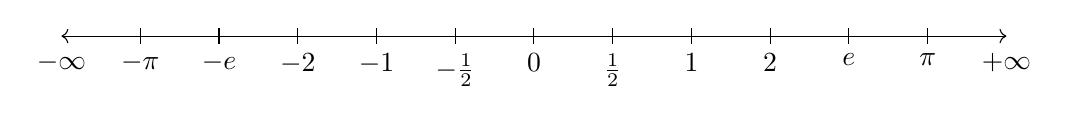
\begin{tikzpicture}
        \draw[->] (0,0) -- (6,0);
        \draw[<-] (-6,0) -- (0,0);
        
        \foreach \x/\label in {-5/{$-\pi$}, -4/{$-e$}, -3/{$-2$}, -2/{$-1$}, -1/{$-\frac{1}{2}$}, 0/{$0$}, 1/{$\frac{1}{2}$}, 2/{$1$}, 3/{$2$}, 4/{$e$}, 5/{$\pi$}} {
            \draw (\x,0.1) -- (\x,-0.1) node[below] {\label};
        }
        \node[below] at (-6,-0.1) {$-\infty$};
        \node[below] at (6,-0.1) {$+\infty$};
    \end{tikzpicture}
\end{center}

\subsection{Exercises}
1) $\forall a,b,x \in \mathbb{R},\ a \leq x \leq b$

\begin{center}
    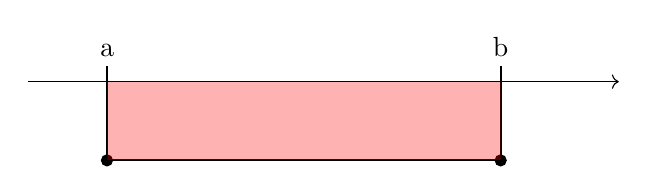
\begin{tikzpicture}
        %number line
        \draw[-] (-4,0) -- (3,0);
        \draw[thick] (-3,-0.2) -- (-3,0.2);
        \draw[thick] (2,-0.2) -- (2,0.2);
        
        %interval
        \draw[thick] (-3,-1) -- (2,-1);
        \draw[thick] (-3,0) -- (-3,-1);
        \draw[thick] (2,0) -- (2,-1);
        \filldraw[black] (-3,-1) circle (2pt);
        \filldraw[black] (2,-1) circle (2pt);
        
        %points
        \node[above] at (-3,0.2) {a};
        \node[above] at (2,0.2) {b};
        
        %arrow
        \draw[->] (3,0) -- (3.5,0);

        %area
        \filldraw [fill=red, draw=black, opacity=0.3] (-3,0) rectangle (2,-1);
    \end{tikzpicture}
\end{center}

2) $\forall x \in \mathbb{R},\ x \in\ ]-2,-1]\ \cup\ ] \frac{3}{2}, +\infty[$

\begin{center}
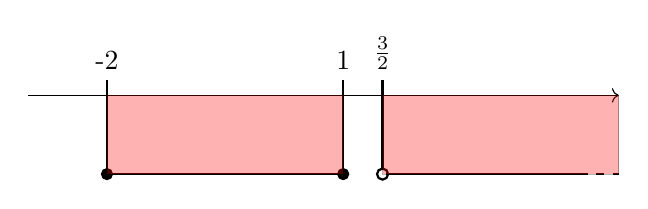
\begin{tikzpicture}
    %number line
    \draw[-] (-3,0) -- (4,0);
    \draw[thick] (-2,-1) -- (-2,0.2);
    \draw[thick] (1,-1) -- (1,0.2);
    \draw[thick] (1.5,-0.95) -- (1.5,0.2);
    
    %intervals
    \draw[thick] (-2,-1) -- (1,-1);
    \filldraw[black] (-2,-1) circle (2pt);
    \filldraw[black] (1,-1) circle (2pt);
    \draw[thick] (1.55,-1) -- (4,-1);
    \draw[thick, dashed] (4,-1) -- (4.5,-1);
    \draw[thick] (1.5,-1) circle (2pt);
    
    %points
    \node[above] at (-2,0.2) {-2};
    \node[above] at (1,0.2) {1};
    \node[above] at (1.5,0.2) {\(\frac{3}{2}\)};
    
    %arrow
    \draw[->] (4,0) -- (4.5,0);

    %area
    \filldraw [fill=red, draw=black, opacity=0.3] (-2,0) rectangle (1,-1);
    \filldraw [fill=red, draw=black, opacity=0.3] (1.5,0) rectangle (4.5,-1);
\end{tikzpicture}
\end{center}
\vspace*{.5cm}
\underline{Notation}: The union of two or more intervals where $x \in \mathbb{R}$
is denoted by the symbol $\cup$.

\newpage
\section{Properties of real numbers}
\subsection{Property 1 - Closure under ``$+$'' and ``$\cdot$''}
$\forall x,y \in \mathbb{R}\\
x+y \in \mathbb{R}\\    
x \cdot y \in \mathbb{R}$

\underline{Remark}: for $\forall x \in \mathbb{Z}$, closure does not hold for division.

\subsection{Property 2 - Commutativity}
$\forall x,y \in \mathbb{R}\\
x+y=y+x\\
x \cdot y=y \cdot x$

\underline{Remark}: commutativity does not hold for divisions and
subtractions.

\subsection{Property 3 - Associative}
$\forall x,y,z \in \mathbb{R}\\
x+(y+z) = (x+y)+z\\
x \cdot (y\cdot z)=(x\cdot y)\cdot z$

\underline{Remark}: associativity does not hold for divisions and
subtractions.

\subsection{Property 4 - Distributive}
$\forall x,y,z \in \mathbb{R}\\
x(y \pm z)=xy \pm xz$

\subsection{Property 5 - Identity}
$\forall x \in \mathbb{R}$
\begin{enumerate}[label=\alph*)]
    \item $0+x=x$
    \item $1 \cdot x=x$
\end{enumerate}

\underline{Remark}: $\forall x \in \mathbb{R},\ x \cdot 0=0$ is
\underline{not} an identity property.

\subsection{Property 6 - Inverses and opposites}
$\forall x \in \mathbb{R}$
\begin{enumerate}[label=\alph*)]
    \item $x+(-x)=0$ (additive inverse)
    \item when $x \neq 0,\ x \cdot \frac{1}{x}=1$ (multiplicative inverse or opposite)
\end{enumerate}

\underline{Remark 1}: $\forall x \in \mathbb{N}$ does not exist either
inverse nor opposite.

\underline{Remark 2}: $\forall x \in \mathbb{Z}$ has inverses, but
not opposites.

\section{The order of operations}
\begin{enumerate}
    \item Perform all operations inside grouping symbols beginning with the innermost set:\\
        $\left(\phantom{-}\right)$ inside brackets operations;
    \item Perform all exponential operations as you come to them, moving left-to-right:\\
        $x^a$;
    \item Perform all multiplications and divisions as you come to them, moving left-to-right:\\
        ``$\cdot$'' and ``$\div$'';
    \item Perform all additions and subtractions as you come to them, moving left-to-right:\\
        ``$+$'' and ``$-$'';
    \item When the level of priority is the same (e.g. multiplications and divisions) solve them as you come to them.
\end{enumerate}

\section{Signed numbers}
A number is denoted as positive if it is directly preceded by a $+$ sign or no sign at all.\\
A number is denoted as negative if it is directly preceded by a $-$ sign.

$\forall x \in \mathbb{R}$
\[-(-x)=x\\
+(-x)=-x\\
+(+x)=x\\
-(+x)=-x\]

\section{Absolute value}
Let $x \in \mathbb{R}$, then

$|x|=$
$\begin{cases}
    x \qquad \text{if } x \geq 0\\
    -x \;\quad \text{if } x < 0
\end{cases}$

\subsection{Property}
$\forall x \in \mathbb{R}\\
|x|>0 \quad \text{if } y \neq 0\\
|x|=0 \quad \text{if } x=0$

\newpage
\part{Lesson 3}
\section{Polynomials}
\subsection{Terms and factors}
\subsubsection{Variables}
A variable is a letter or a symbol that can assume any value.
\figbox{$\forall x \in \mathbb{R}$}\\
The most common variables are $a$, $b$, $x$, $y$.

When we have an equality $y=x+a$, $\forall x \in \mathbb{R}$, $x$ can assume
any value in the set of real numbers ($x$ is an independent variable), while $y$ strictly depends on the
value that we decide to give to x. 

\underline{Notice}: we can write $y=x+a$ as $y-a=x$, changing which variable is
independent and which is dependent.

\subsubsection{Sets}
Consider the set $A=\left[a,b\right]$, where $a \leq b$. Then:
\figbox{$\forall x \in A, \; a \leq x \leq b$}

\subsection{Expressions, terms and factors}
\subsubsection{Expressions}
An expression is any formula containing numbers, variables, operations, and
brackets.
\figbox{$y=ax^2+bx\cdot c$}

\subsubsection{Terms}
A term is any part of the expression separated by ``$+$'' or ``$-$''.
\figbox{$y = \underbrace{ax^2}_{term} + \underbrace{bx \cdot c}_{term}$}

\subsubsection{Factors}
Each term can be split into a product of factors.
\figbox{$x \cdot y \cdot (a-b) \cdot 24 = x \cdot y \cdot (a-b) \cdot 2 \cdot 2 \cdot 2 \cdot 3$}

\underline{Notice}: the process of splitting a term into several factors is called ``factorization''.\\
\phantom{} \hspace{1cm} The goal of a factorization is to factorize an expression as much as possible.

\newpage
\section{Common factor}
Any expression made of terms is composed of several factors.
\figbox{$x^2+x^3+x= x(x+x^2+1),\ \forall x \in \mathbb{R}$}

\section{Notable products}
\begin{itemize}
    \item $(a+b)^2=a^2+2ab+b^2$ (difference of two squares);
    \item $(a-b)^2=a^2-2ab+b^2$ (square of a binomial);
    \item $(a-b)(a+b)=a^2-b^2$ (difference of squares);
    \item $(a-b)(a^2+b^2+ab)=a^3-b^3$ (difference of two cubes);
    \item $(a+b)(a^2+b^2-ab)=a^3+a^3$ (sum of cubes).
\end{itemize}

\underline{Remark}: notable products are useful to factorize expressions when we don't know a common factor.

\section{Classification of polynomials}
Polynomials can be classified using two criteria: 
\begin{enumerate}
    \item the number of terms;
    \item the degree of the polynomial.
\end{enumerate}
\begin{equation}
    \begin{aligned}
        &\begin{array}{|c|c|l|c|}
        \hline \text { Number of Terms } & \text { Name } & \text { Example } & \text { Comment } \\
        \hline \text { One } & \text { Monomial } & ax^2 & \text { Mono means ``one'' in Greek } \\
        \hline \text { Two } & \text { Binomial } & ax^2-b x & \text { Bi means ``two'' in Latin } \\
        \hline \text { Three } & \text { Trinomial } & ax^2-b x+c & \text { Tri means ``three'' in Greek } \\
        \hline \text { Four or more } & \text { Polynomial } & a x^3-b x^2+c x-d & \text { Poly means ``many'' in Greek } \\
        \hline
        \end{array}
    \end{aligned}
\end{equation}

\subsection{Definition}
Let $n \in \mathbb{N^*}$, then a polynomial is the sum or difference of n-monomials. 

\subsection{Degree}
The degree of a polynomial is the largest exponent of its monomials.

\subsubsection{Monomials}
The degree of a monomial is the sum of all the exponents of all the variables.

$p(x)=x^2+1 \rightarrow$ the degree is 2.\\
$\forall x \in \mathbb{R},\ p(0)=0^2+1=1 \rightarrow$ 1 is a polynomial with degree 0.

\subsubsection{Polynomials}
The degree of a polynomial is the highest of all the degrees of all the
monomials which compose the polynomial.

$p(x)=x^3+1+x^5+x^21 \rightarrow \deg(p(x))=21$\\
$q(x)=12 \underbrace{abcd}_{\deg=4} - 31x^3+2xy \rightarrow \deg(q(x))=4$ 

\underline{Notation}: Let $f(x)=ax^2+bx+c$, $a$ and $b$ are called coefficient.\\
The coefficient of the monomial with highest coefficient is called \textbf{leading coefficient}.

\newpage
\part{Lesson 4}
\section{Operations between polynomials}
\subsection{Polynomials with one independent variable}
The order of the monomials is not important, but it is preferable to write
the highest degree monomials in decreasing order.
\figbox{$p(x)=ax^2-bx+c$}

\subsubsection{Sum}
We have to sum all the monomials of the same degree.

$p(x)=x^2+x-1\\
q(x)=5-x+x^5-x^2$

$p(x)+q(x)=x^2+x-1+5-x+x^5-x^2=x^5+4$

\underline{Definition}: in a polynomial with one variable, monomials of same
degree are called \textbf{similar terms}.

\underline{Remark}: when there is a difference between polynomials, the minus MUST be distributed throughout the next monomial.

\subsubsection{Multiplications}
We have to multiply the factors with each other using the distributive property.

$p(x)=(x-1)\\
q(x)=(x^2+2x)$

$p(x)\cdot q(x)=(x-1)(x^2+2x)=x^3+2x^2-x^2-2x=x^3+x^2-2x=x(x^2+x-2)$

\subsection{Polynomials with two or more variables}
\subsubsection{Sum}
$p(x)=ab+a^2b\\
q(x)=4ab-3ab^2$

$p(x)+q(x)=ab+a^2b+4ab-3ab^2=a^2b-3ab^2+5ab=ab(a-b+5)$

\underline{Remark}: $5a^3b^4+7a^3b^4=12a^3b^4$, but with $5a^3b^4+7a^4b^3$ we can't go further with the sum.

\section{Equations}
An equation is a formula given by the equality of expressions.

\underline{Symbol notations}: 
\begin{itemize}
    \item $\exists =$ there exist(s);
    \item $\nexists =$ there does not exists;
    \item $\exists! =$ it exists and it is unique;
    \item $:$ or $| =$ such that.
\end{itemize}

Equations are the main topic, then we have
\begin{itemize}
    \item Identities;
    \item Contradictions;
    \item Conditional equations.
\end{itemize}

\newpage
\subsection{Identities}    
An identity is an equality that holds true regardless of the values chosen for its variables:
\figbox{$\forall x \in \mathbb{R},\ \exists y \in \mathbb{R}\ |\ f(x,y)=0$}\\
e.g.
\begin{itemize}
    \item $1=1$;
    \item $x-1=-1+x$;
    \item $\sin^2(x)+\cos^2(x)=1$.
\end{itemize}
\subsection{Contradictions}
A contradiction occurs when we get a statement $p$, such that $p$ is true and its negation $\sim p$ is also true:
\figbox{$\forall x \in \mathbb{R}, \ \neg (\exists y \in \mathbb{R}\ |\ f(x, y) = 0)$}\\
e.g.
\begin{itemize}
    \item $0=1$, false;
    \item $x^2=-1$ it is always positive or zero;
    \item $|a|=-3$ it is always positive or zero;
    \item $\sqrt{-(x^2+1)}=1$ it is never defined ($\nexists $).
\end{itemize}

\subsection{Conditional equations}
In general, we want to find a solution for each equation, i.e. all the
real numbers that, when they replace a variable inside the equation, give an identity:
\figbox{$\forall x \in \mathbb{R}, \ (x > 0 \Rightarrow \exists y \in \mathbb{R}\ |\ f(x, y) = 0)$}\\
e.g.
\begin{itemize}
    \item $x=1$;
    \item $x+y=3$;
    \item $\sin(\alpha)=0.5$.
\end{itemize}

\section{Fundamental theorem of algebra}
Let $p(x)$ be a polynomial with one variable and real coefficients.\\
Assume that $\deg(p(x))=n \in \mathbb{N}$, then:
\figbox{$p(x)=0$ has at most $n$ solutions}
    
\section{Linear equations with one variable}
$p(x)=q(x)$ where $\deg(0,(x))=1$

\subsection{Simple tools}
\subsubsection{Tool 1}
$a,b \in \mathbb{R},\ x+a=b$, let's isolate the variable $x$: $x-a-a=b-a \Rightarrow x=b-a$

\subsubsection{Tool 2}
$a,b \in \mathbb{R},\ ax=b$, let's isolate the variable $x$: $\frac{ax}{a}=\frac{b}{a} \Rightarrow x=\frac{b}{a}$

\newpage
\section{Linear inequalities with one variable}
The inequality is a relation between two or more sets.\\
Let $a,b,x \in \mathbb{R},\ a<x,\ b>x$, then:
\figbox{$a<x<b$}

\subsection{Negative sign}
In solving the inequality we have to move a negative factor from one side to the other,
so we need to reverse the sign of the inequality:
\figbox{$-ax<b \Rightarrow x>-\frac{b}{a}$}

\section{Equations and inequalities with absolute values}
To solve absolute values we need to consider two cases.\\
Let's take this equation: $|x+2|=-x+4$, then
\figbox{$
    \begin{cases}
        \text{case 1: } x+2 = -x+4 \Rightarrow 2x = 2 \Rightarrow x_1 = 1\\
        \text{case 2: } -x-2 = -x+4 \Rightarrow -2 = 4 \ (\text{contradiction})
    \end{cases} \Longrightarrow \text{Sol: } x=
    \begin{cases}
            1\ &\text{ if }\ x+2 \geq 0\\
            \text{no solution} &\text{ if }\ x+2 < 0
    \end{cases}$
}

\newpage
\part{Lesson 5}
\section{Division of polynomials}
\subsection{Division algorithm for polynomials by monomials}
Let $f(x)$ be a polynomial and $g(x)$ a monomial such that $g(x) \neq 0$. Consider the rational expression $\frac{f(x)}{g(x)}$, then:

\begin{center}
    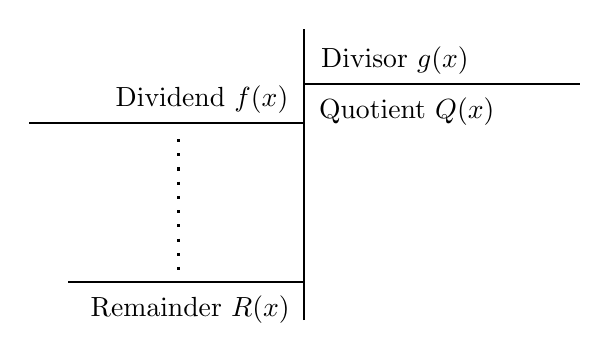
\begin{tikzpicture}
        %vline
        \draw[thick] (0,0) -- (0,3.7);
        %hlines
        \draw[thick] (0,3) -- (3.5,3);
        \draw[thick] (0,2.5) -- (-3.5,2.5);
        \draw[thick] (0,0.48) -- (-3,0.48);
        %dots
        \draw[line width=0.4mm, loosely dotted] (-1.6,2.3) -- (-1.6,0.6);

        %nodes
        \node at (1.15,3.3) {Divisor $g(x)$};
        \node at (-1.3,2.8) {Dividend $f(x)$};
        \node at (1.3,2.65) {Quotient $Q(x)$};
        \node at (-1.45,0.13) {Remainder $R(x)$};
    \end{tikzpicture}
\end{center}

\begin{itemize}
    \item Divide the highest degree term in $f(x)$ (the dividend) by the highest degree term in $g(x)$ (the divisor). This gives the first partial quotient $q_1(x)$.
    \item Multiply the partial quotient $R_1(x)$ by the entire divisor $g(x)$. This product represents the part of the dividend that can be "cancelled" in this step.
    \item Subtract the product obtained in step 2 from the original dividend $f(x)$. This subtraction gives a new polynomial, often called the remainder $R_1(x)$, which is of a lower degree than the original dividend.
    \item Now divide the leading term of the new remainder $R_1(x)$ by the leading term of $g(x)$. This gives the next partial quotient $Q_2(x)$.
    \item Multiply $Q_2(x)$ by $g(x)$ and subtract it from the current remainder. This process generates a new remainder $R_2(x)$.
    \item Keep repeating the division, multiplication, and subtraction steps until the degree of the remainder is less than the degree of the divisor $g(x)$. At this point, you cannot continue dividing.
    \item The final quotient $Q(x)$ is the sum of all the partial quotients: $Q(x) = Q_1(x) + Q_2(x) + \dots + Q_n(x)$.
    \item The remainder $R_n(x)$ is the result after all subtractions are completed. If the remainder is zero, the division is exact. If not, the remainder is the leftover part of the division.
\end{itemize}\

\underline{Tip}: When the sum of the coefficients is equal to 0, then the polynomial is always divisible by $x-1$.

\section{Second degree polynomials}
Let $a,b,c \in \mathbb{R}$, with $a \neq 0$, then
\figbox{$ax^2+bx+c=0$}

The three possible outcomes we can have when solving this 2nd-degree polynomial are:
\begin{itemize}
    \item 2 solutions;
    \item 1 solution;
    \item 0 solutions.
\end{itemize}

\subsection{Quadratic formula}
\figbox{$x_{1,2}=\frac{-b \mp \sqrt{\Delta}}{2a}$}

\subsubsection{Discriminant of the polynomial}
\figbox{$\Delta=b^2-4ac$}

From the discriminant we can determine how many solutions the equation will have:
\begin{itemize}
    \item $\Delta>0 \Rightarrow 2$ real solutions;
    \item $\Delta=0 \Rightarrow 1$ real solution;
    \item $\Delta<0 \Rightarrow 0$ real solutions (2 complex solutions).
\end{itemize}

\subsubsection{Evident solutions}
When we have a 2nd-degree equation $(x-a)(x-b)=0$, we have two obvious solutions
in $\mathbb{R}$. In this case, $x_1=a,\ x_2=b$ 

This factorization can be obtained using notable products.

e.g. Let $x^2+4x+4=0 \Rightarrow (x+2)^2=0$, then $x=-2$.

\subsection{Extraction of a root}
Let $a \in \mathbb{R},\ a\geq 0$, then:
\figbox{$x^2-a=0 \Rightarrow x=\pm\sqrt{a}$}

\newpage
\part{Lesson 6}
\section{Lines and parabolas}
\subsection{Cartesian diagram}
\begin{center}
    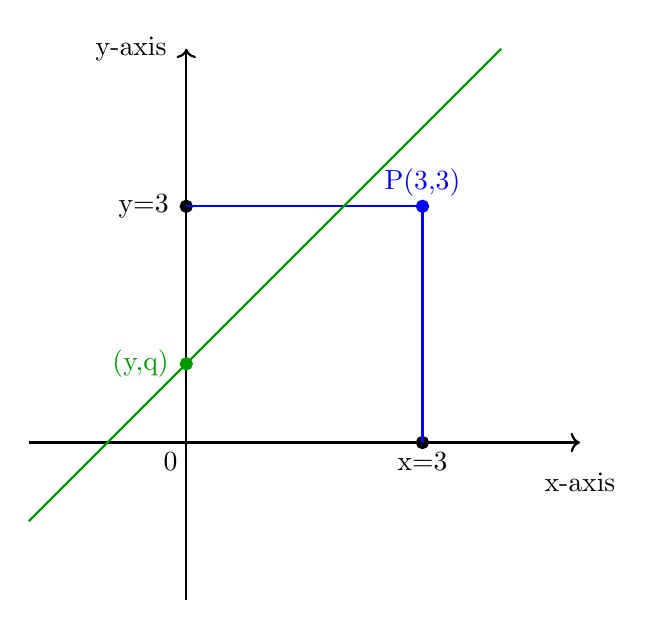
\begin{tikzpicture}
        \definecolor{darkgreen}{rgb}{0.0, 0.6, 0.0}

        \draw[thick][->] (-2,0) -- (5,0);
        \draw[thick][->] (0,-2) -- (0,5);
        \node at (5,-.5) {x-axis};
        \node at (-.7,5) {y-axis};
        \draw[fill, thick] (3,0) circle (2pt);
        \node[below] at (3,0) {x=3};
        \draw[fill, thick] (0,3) circle (2pt);
        \node[left] at (-.1,3) {y=3};
        \draw[blue, thick] (3,0) -- (3,3);
        \draw[blue,thick] (0,3) -- (3,3);
        \draw[fill, blue, thick] (3,3) circle (2pt);
        \node[blue, above] at (3,3) {P(3,3)};
        \node[below] at (-0.2,0) {0};
        
        \draw[darkgreen, thick] (-2,-1) -- (4,5);
        \draw[fill, darkgreen, thick] (0,1) circle (2pt);
        \node[darkgreen, left] at (-0.1,1) {(y,q)};

    \end{tikzpicture}
\end{center}

\subsection{Straight line}
Let A and B be any two distinct points, then there is one and only one
line passing through A and B.

\subsection{Slope-intercept equation}
Let $m,q \in \mathbb{R}$, then
\figbox{$y=mx+q$}

\begin{itemize}
    \item $m$: slope ($\tan(\alpha)$);
    \item $q$: vertical intercept.
\end{itemize}

\subsubsection{Slope}
The slope of a line can be calculated with the equation
\figbox{$m=\frac{y_B - y_A}{x_B - x_A} = \frac{\Delta y}{\Delta x}$}

We have three different slope outcomes:
\begin{itemize}
    \item $m>0$, the line is increasing;
    \item $m=0$, the line is stable;
    \item $m<0$, the line is decreasing. 
\end{itemize}

\newpage
\subsubsection{Drawing}
\begin{center}
    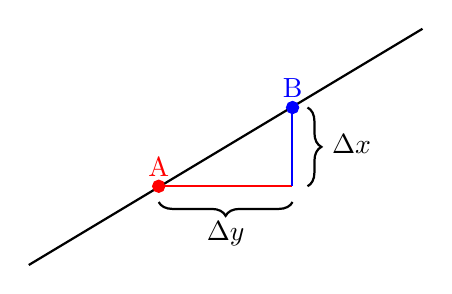
\begin{tikzpicture}
        \draw[thick] (0,0) -- (5,3);
        \draw[fill, thick, red] (1.65,1) circle (2pt);
        \node[above, red] at (1.65,1) {A};
        \draw[fill, thick, blue] (3.35,2) circle (2pt);
        \node [above, blue] at (3.35, 2) {B};

        %slope
        \draw[thick, red] (1.65,1) -- (3.34,1);
        \draw[thick, blue] (3.34,2) -- (3.34,1);

        %braces
        \draw[decorate,decoration={brace,amplitude=5pt},thick] (3.54,2) -- (3.54,1);
        \node at (4.1,1.53) {$\Delta x$};
        \draw[decorate,decoration={brace,amplitude=5pt},thick] (3.35,0.8) -- (1.65,0.8);
        \node at (2.5,0.4) {$\Delta y$};
    \end{tikzpicture}
\end{center}

\subsection{Vertical lines}
The more the value of m increases, the closer the line will get to the vertical,
without ever reaching it.

Let $c \in \mathbb{R}$, then $x=c$.

Vertical lines cannot be written as a function.

\section{Equation of a line}
Let $m,x_A,y_A \in \mathbb{R}$ and $A(x_A, y_A)$, then
\figbox{$y-y_A=m(x-x_A)$}

e.g.: Find the line with $m=-1$ and $A(2,-1)$.
\[
    y-1=-1(x+2) \Rightarrow y=-x+1
\]
\hspace{.75cm} Points: $A(2,-1);\ B(0,1)$


\begin{center}
    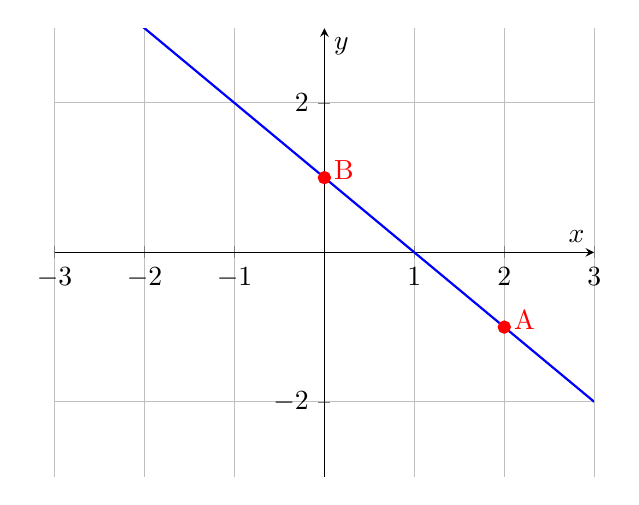
\begin{tikzpicture}
        \begin{axis}[
                axis lines = middle,
                xlabel = $x$,
                ylabel = $y$,
                grid = both,
                xmin=-3, xmax=3,
                ymin=-3, ymax=3,
                domain=-3:3
            ]
            \addplot[color=blue, thick] {-x + 1};
            \draw[fill, red, thick] (2,-1) circle (2pt);
            \node[right,red] at (2,-.9) {A};
            \draw[fill,red,thick] (0,1) circle (2pt);
            \node[right,red] at (0,1.1) {B};
        \end{axis}
    \end{tikzpicture}
\end{center}

\subsection{General equation in a cartesian diagram}
\figbox{$ax+by+c=0$}

\underline{Remarks}:
\begin{itemize}
    \item All the lines can be described with this kind of equation;
    \item When $b=0$, $a \neq 0$, then $ax=-c \Rightarrow x=\frac{-c}{a} \in \mathbb{R}$;
    \item When $b \neq 0$, then $y=-\frac{a}{b}x -\frac{c}{b}$,
        where $m=-\frac{a}{b}$ and $q=-\frac{c}{b}$.
\end{itemize}

\newpage
\section{Vertical parabolas}
\subsection{Function of parabolas}
Let $a,b,c \in \mathbb{R}$, then
\figbox{$y=a^2+bx+c$}

\subsection{Drawing example}
\vspace*{0.8cm}
\begin{wrapfigure}{r}{10cm}
    \vspace*{-2.75cm}
    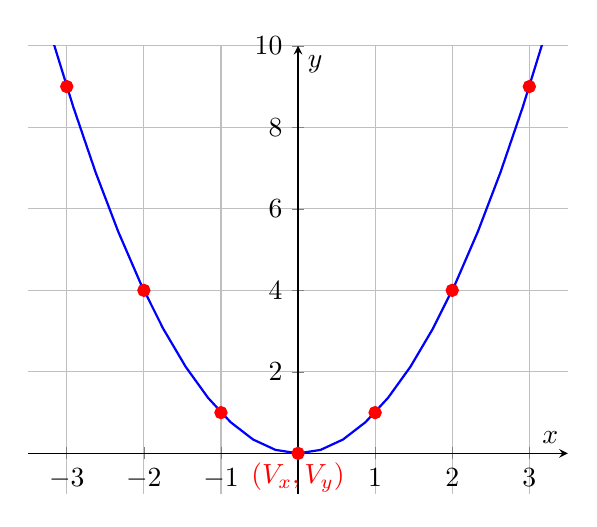
\begin{tikzpicture}
        \begin{axis}[
            axis lines = middle,
            xlabel = $x$,
            ylabel = $y$,
            grid = both,
            xmin=-3.5, xmax=3.5,
            ymin=-1, ymax=10,
            domain=-3.5:3.5
        ]
        \addplot[color=blue, thick] {x^2};
        \draw[fill,red,thick] (-3,9) circle (2pt);
        \draw[fill,red,thick] (-2,4) circle (2pt);
        \draw[fill,red,thick] (-1,1) circle (2pt);
        \draw[fill,red,thick] (-0,0) circle (2pt);
        \node[red, below] at (0,0) {$(V_x, V_y)$};
        \draw[fill,red,thick] (1,1) circle (2pt);
        \draw[fill,red,thick] (2,4) circle (2pt);
        \draw[fill,red,thick] (3,9) circle (2pt);
        \end{axis}
    \end{tikzpicture}
\end{wrapfigure}
\hspace*{2.25cm}
\begin{tabular}{c|c}
    x & y \\ \hline
    -3 & 9 \\
    -2 & 4 \\
    -1 & 1 \\
    0 & 0 \\
    1 & 1 \\
    2 & 4 \\
    3 & 9  
\end{tabular}
\vspace*{-2cm}
\wrapfill

\subsection{Concavity of a parabola}
We have three cases:
\begin{itemize}
    \item $a>0$, concave up;
    \item $a=0$, not a parabola;
    \item $a<0$, concave down.
\end{itemize}

\subsection{Vertex of a parabola}
The vertex of a parabola $y=ax^2+bx+c$ is the point given by the coordinates:
\figbox{$V=\left(-\frac{b}{2a},\ -\frac{\Delta}{4a}\right)$}

\underline{Remarks}: we have two different cases:
\begin{itemize}
    \item When $a>0$, the vertex is the lower point of the parabola;
    \item When $a<0$, the vertex is the highest point of the parabola.
\end{itemize}

e.g.: given $y=x^2$, find the vertex:
$V=\left(-\frac{0}{2},\ -\frac{0}{4}\right) \rightarrow V(0,0)$

\underline{Alternative}: solving the $x$ coordinate $V_x$, we can
sostitute the $x$ inside the given funcion $f(x)$.

\newpage
\section{Powers with $\mathbb{Z}$ and $\mathbb{R}$ exponents}
Let $\alpha \in \mathbb{R}$ and $n \in \mathbb{N}$, then:
\figbox{$\alpha^{\frac{1}{n}}=\sqrt[n]{\alpha}$}

Let $m,n \in \mathbb{Z}$, then
\figbox{$\alpha^{\frac{m}{n}}=\left(\alpha^\frac{1}{n}\right)^m$}

Let $a,c \in \mathbb{Z};\ b,d \in \mathbb{Z}^*$ and $\lambda \in \mathbb{R} \difference \mathbb{Z}$. Then, we can approximate $\lambda$
by a fraction:

\figbox{$\frac{a}{b}<\lambda<\frac{c}{d}$}

\newpage
\part{Lesson 7}
\section{Concept of functions}
Let's take any two sets $A\left\{a,b,c,d,e,f,g\right\}$ and $B\left\{a_1,b_1,c_1,d_1,e_1,f_1,g_1\right\}$.

\figbox{ \hspace*{-1cm}
    \begin{minipage}{0.12\textwidth}
        \vspace*{-0.4cm}
        \begin{align*}
            f: \mathbb{R} &\longmapsto \mathbb{R} \\
            x &\longmapsto mx+q
        \end{align*}
    \end{minipage}
}

A function is a relation between the sets $A$ and $B$, according to which we
associate to each element of $A$ one and only one element of $B$:

\figbox{
    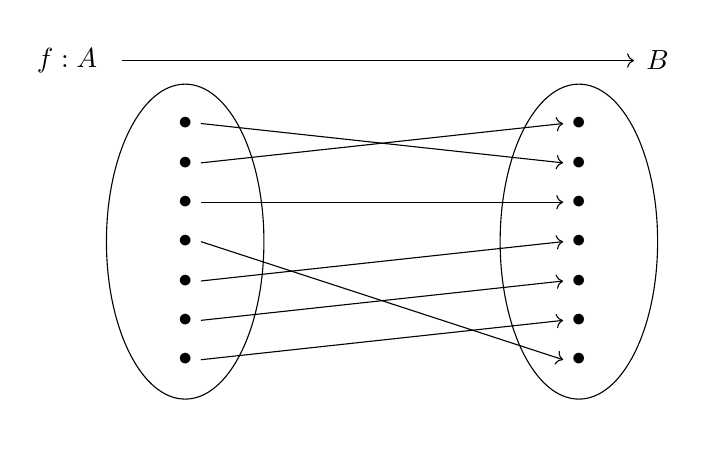
\begin{tikzpicture}
        %sets A and B
        \draw (0,0) ellipse (1 and 2);
        \draw (5,0) ellipse (1 and 2);
        \node at (-1.5,2.3) {$f:A$};
        \node at (6,2.3) {$B$};
        \draw[->] (-0.8,2.3) -- (5.7,2.3);
        
        %set A
        \node at (0,-1.5) {$\bullet$};
        \node at (0,-1) {$\bullet$};
        \node at (0,-0.5) {$\bullet$};
        \node at (0,0) {$\bullet$};
        \node at (0,0.5) {$\bullet$};
        \node at (0,1) {$\bullet$};
        \node at (0,1.5) {$\bullet$};
        
        %set B
        \node at (5,-1.5) {$\bullet$};
        \node at (5,-1) {$\bullet$};
        \node at (5,-0.5) {$\bullet$};
        \node at (5,0) {$\bullet$};
        \node at (5,0.5) {$\bullet$};
        \node at (5,1) {$\bullet$};
        \node at (5,1.5) {$\bullet$};
        
        %arrows
        \draw[->] (0.2,-1.5) -- (4.8,-1);
        \draw[->] (0.2,-1) -- (4.8,-0.5);
        \draw[->] (0.2,-0.5) -- (4.8,0);
        \draw[->] (0.2,0) -- (4.8,-1.5);
        \draw[->] (0.2,0.5) -- (4.8,0.5);
        \draw[->] (0.2,1) -- (4.8,1.5);
        \draw[->] (0.2,1.5) -- (4.8,1);

        %spacer
        \node at (0,2.6) {\phantom{}};
        \node at (0,-2.2) {\phantom{}};
    \end{tikzpicture}
}

Each point in set $B$ is reached by at least one arrow. However, it is
possible for more than two elements of $A$ to point to the same element of $B$.

\section{Trigonometry}
Trigonometric functions can be extended to angles beyond 0 and 90$^\circ$
using the unit circle. For an angle $\theta$ in the unit circle:
\figbox{$\sin \theta = y\ \ |\ \cos \theta = x\ \ |\ \tan \theta = \frac{y}{x}$}

\subsection{Conversion table of degrees and radians}
\begin{center}
    \begin{tabular}{|c|c|c|c|c|c|c|c|c|}
        \hline
        \textbf{Angles (in Degrees)} & \rule{0pt}{15pt} $0^\circ$ & $30^\circ$ & $45^\circ$ & $60^\circ$ & $90^\circ$ & $180^\circ$ & $270^\circ$ & $360^\circ$ \\
        \hline
        \textbf{Angles (in Radians)} & \rule{0pt}{15pt} $0$ & $\pi/6$ & $\pi/4$ & $\pi/3$ & $\pi/2$ & $\pi$ & $3\pi/2$ & $2\pi$ \\
        \hline
        $\sin(\theta)$ & \rule{0pt}{15pt} 0 & $1/2$ & $\sqrt{2}/2$ & $\sqrt{3}/2$ & 1 & 0 & $-1$ & 0 \\
        \hline
        $\cos(\theta)$ & \rule{0pt}{15pt} 1 & $\sqrt{3}/2$ & $\sqrt{2}/2$ & $1/2$ & 0 & $-1$ & 0 & 1 \\
        \hline
        $\tan(\theta)$ & \rule{0pt}{15pt} 0 & $\sqrt{3}/3$ & 1 & $\sqrt{3}$ & $\infty$ & 0 & $\infty$ & 0 \\
        \hline
    \end{tabular}
\end{center}
\phantom{}

\underline{Remark}:

\begin{center}
    $\cos(360^{\circ}+\theta) = \cos(\theta) \qquad | \qquad
    \sin(360^{\circ}+\theta) = \sin(\theta)$
\end{center}


\underline{Remark}:
Let $\forall k \in \mathbb{Z},\ \forall \theta \in \mathbb{R}$, then:
\figbox{$\cos(\theta + k\cdot360^{\circ})=\cos(\theta)$}

\newpage
\subsection{Trigonometric functions in the unit circle}
\begin{center}
    \begin{tikzpicture}[scale=3.75]
        \definecolor{darkgreen}{rgb}{0.0, 0.7, 0.0}
        % Draw the x and y axes
        \draw[thick, ->] (-1.5,0) -- (1.5,0) node[right] {$x$};
        \draw[thick, ->] (0,-1.5) -- (0,1.5) node[above] {$y$};
    
        % Draw the unit circle
        \draw (0,0) circle (1);
    
        % Draw the angle theta
        \draw[thick, blue] (0,0) -- (0.866,0.5) node[right] {$P(x,y)$};
        \draw[dashed, blue] (0,0) -- (0.866,-0.5) node[right] {\ $P'(x,y')$};
    
        % Draw dashed lines to indicate the projections on the axes
        \draw[dashed] (0.866,-0.5) -- (0.866,0.5) -- (0,0.5);
    
        % Label the angle theta
        \draw (0.3,0) arc (0:30:0.3);
        \node at (0.35,0.10) {$\theta$};
    
        % Label the origin
        \node at (-0.06, -0.06) {$O$};
    
        % Draw the projections on the axes
        \draw[thick, red] (0,0) -- (0.866, 0) node[midway, below] {$\cos \theta$};
        \draw[thick, darkgreen] (0,0) -- (0, 0.5) node[midway, left] {$\sin \theta$};
    
        % Additional labels and lines
        \node at (1.075, 0.05) {1};
        \node at (-0.05, 1.1) {1};
        \node at (-1.075, 0.05) {-1};
        \node at (-0.05, -1.1) {-1};
    
        % Labels for each quadrant
        \node at (1, 1) {I};
        \node at (-1, 1) {II};
        \node at (-1, -1) {III};
        \node at (1, -1) {IV};

        %others
        \draw (0.866,0) rectangle (0.816,0.05);
        \node[below] at (0.93,0) {$H$};

        %braces
        \draw[decorate,decoration={brace,amplitude=5pt},thick] (1.65,0.5) -- (1.65,-0.5);
        \node at (1.9,0) {$\Delta y = 1$};
    \end{tikzpicture}
\end{center}

\subsubsection{Property 1}
Because we are inside a circle of radius 1:
\begin{itemize}
    \item $-1 \leq \cos(\theta) \leq 1$;
    \item $-1 \leq \sin(\theta) \leq 1$.
\end{itemize}

\subsubsection{Property 2}
Because we have a 90$^\circ$ angle, we can use Pythagoras: 
\figbox{$\vv{OH}^{\,2}+\vv{PH}^{\,2}=\vv{OP}^{\,2}$}

Then, we can compute that:
\figbox{$\sin^2(\theta) + \cos^2(\theta) = 1 \qquad \forall\, \theta \in \mathbb{R}$}

\subsubsection{Example with 45$^{\circ}$}
When $\theta=45^{\circ}$, then $\sin(\theta)=\cos(\theta) \Rightarrow 2\cos^2(\theta)=1
\Rightarrow \cos(\theta)=\sqrt{\frac{1}{2}} \Rightarrow \sin(\theta)=\cos(\theta)=\frac{\sqrt{2}}{2}$

\subsection{Tangent}
A tangent of an angle is exactly the slope of a line:
\figbox{$m = \frac{\Delta y}{\Delta x} = \tan(\theta)=\frac{\sin(\theta)}{\cos(\theta)}$}

\underline{Remark}: the tangent is not defined when the angle is 90$^{\circ}$
or 270$^{\circ}$, that is when we have a vertical line.

\end{document}